% \pending{...} and \tbd mark results still to come; both print in bold brackets.
\providecommand{\pending}[1]{\textbf{[PENDING: #1]}}
\providecommand{\tbd}{\textbf{[PENDING]}}

\chapter{Results and Discussion}
\begin{refsection}
This chapter presented and discussed the results of the evaluation of ThemeSync. After the evaluation setup, one section covered each specific objective. Each table and figure was followed by its results and by a discussion of the principal findings, their interpretation, the related literature, the implications, the limitations, and a summary.

\section{Evaluation Setup}

The evaluation used four sets of data, each matched to its metrics (\ref{tab:eval-sets}). The deployed system used the YOLOv8s layout detector trained on the empirical master-layout dataset, the third version of the Graph Neural Network (GNN), the Cassowary constraint solver, and the Heuristic Fitness Function (Formula 3.11) with weights $\alpha = 50$, $\beta = 2$, $\gamma = 1$, and $\delta = 1.5$.

\begin{table}[H]
\centering
\caption{Evaluation Sets and the Metrics Computed on Them}
\label{tab:eval-sets}
\begin{tabular}{>{\raggedright\arraybackslash}p{0.30\textwidth} >{\raggedright\arraybackslash}p{0.26\textwidth} >{\raggedright\arraybackslash}p{0.34\textwidth}}
\hline
\textbf{Set} & \textbf{Size} & \textbf{Metrics} \\ \hline
Validation split of the empirical master-layout dataset & 40 images, 607 annotated elements & Intersection over Union (IoU), mAP50 \\
Held-out CGL-Dataset layouts (a seeded 5\% of the training split) & 2,900 layouts & GNN position, gap, and order errors \\
Unseen event posters (purposive sample, in no training set) & 16 posters $\times$ 2 formats & Structure error, Heuristic Fitness Function, F1-score, latency, MOS \\
Synthetic administrative templates & Certificate and event ID, 52 runs & Stress test: F1-score, reading order, text fit \\ \hline
\end{tabular}
\end{table}

Three Stage 2 conditions were compared on the unseen posters. \textit{Structure mapping + GNN} was the full system: the target elements were mapped to the master's structure and then refined by the GNN. \textit{Structure mapping only} turned the GNN off to isolate its contribution. The \textit{baseline} used neither and stacked the elements in reading order. All three shared the archetype chosen from the master's composition, the palette, the background, and the stylistic markers. Phase 4 compared structure mapping + GNN with the baseline.

The Phase 3 battery (16 posters $\times$ 2 formats $\times$ 3 conditions, 96 runs) ran on the school's server (Python 3.10, PyTorch 2.5.1, Ultralytics 8.4) with an NVIDIA RTX A5000 GPU (24 GB). The detector's IoU, the stress test, the latency benchmark, and the check of the rated layouts ran on a workstation with an NVIDIA RTX 3060 GPU (Python 3.12, PyTorch 2.5.1) with the same model libraries.
% Sources: results/experiment_log.json (run 20261006_195534); results/yolo_iou.json;
% results/stress_test.json; results/latency_benchmark.json; results/rated_layouts_check.json.

% =====================================================================
\clearpage
\section{Objective 1: Relational Logic and Feature Extraction}

The first specific objective was to design a Relational Logic and Feature Extraction model that integrated the GNN, K-Means clustering, and SIFT to identify and map the structural dependencies and stylistic markers of master design files.

\subsection{Semantic Layout Parsing}

\ref{tab:domain-gap} presented the highest detection confidence of the first three detectors on three real event posters outside their training sets.

\begin{table}[H]
\centering
\caption{Highest Detection Confidence on Three Real Posters Outside the Training Sets}
\label{tab:domain-gap}
\begin{tabular}{l c c c}
\hline
\textbf{Detector} & \textbf{La Serata} & \textbf{TAN-AW} & \textbf{LODT} \\ \hline
v1 (CGL-Dataset only) & 0.035 (0) & 0.204 (0) & 0.211 (0) \\
v2 (+ 65 master layouts) & 0.740 (16) & 0.735 (13) & 0.694 (8) \\
v3 (+ 124 master layouts) & 0.843 (10) & 0.753$^{a}$ (9) & 0.793 (11) \\ \hline
\multicolumn{4}{p{0.80\textwidth}}{\footnotesize Values in parentheses are the number of detections at or above the 0.25 confidence threshold. $^{a}$TAN-AW was part of v3's training data.}
\end{tabular}
\end{table}
% Source: results/yolo_domain_gap_check.json; v1 in-domain mAP50 0.539 (notes §3.5).

On the CGL-Dataset's own held-out images, v1 reached an mAP50 of 0.539, but on the event posters no detection reached the 0.25 threshold. After fine-tuning on 65 annotated master layouts (v2), each poster produced 8 to 16 detections.

The CGL-trained detector could not read event posters, and a little in-domain data fixed this. The CGL-Dataset's e-commerce posters \cite{zhou2022cglgan} differ from school event posters. dos Santos Júnior, Paixão, and Alvarez [\citeyear{dosSantosJunior2025}] found YOLOv8 effective for the layout analysis of historical documents; here, it worked on event posters only after training on them. A public dataset from another domain cannot be assumed to transfer, so the study built its own. Only three posters were checked. Layout parsing required in-domain data.

\clearpage
The detector was then developed in two more steps (\ref{tab:yolo-dev}). Values were comparable within a panel but not across panels.

\begin{table}[H]
\centering
\caption{Development of the Layout Detector}
\label{tab:yolo-dev}
\begin{tabular}{l c c c c c}
\hline
\textbf{Detector} & \textbf{All} & \textbf{Logo} & \textbf{Text} & \textbf{Underlay} & \textbf{Embellishment} \\ \hline
\multicolumn{6}{l}{\textit{A. mAP50 on the validation labels of the 124-image batch}} \\
v3 (YOLOv8n, 640 px) & 0.363 & 0.620 & 0.584 & 0.037 & 0.212 \\
v4 (YOLOv8s, 1024 px) & 0.454 & 0.818 & 0.682 & 0.115 & 0.201 \\ \hline
\multicolumn{6}{l}{\textit{B. mAP50 on 32 validation images that neither model trained on}} \\
v4 (124 images) & 0.486 & 0.864 & 0.680 & 0.138 & 0.263 \\
v5 (200 images) & 0.728 & 0.977 & 0.684 & 0.643 & 0.609 \\ \hline
\multicolumn{6}{l}{\textit{C. Recall on the same 32 images}} \\
v4 (124 images) & 0.458 & 0.868 & 0.657 & 0.097 & 0.210 \\
v5 (200 images) & 0.671 & 0.938 & 0.722 & 0.516 & 0.507 \\ \hline
\multicolumn{6}{p{0.86\textwidth}}{\footnotesize Panels B and C left out the eight validation images that either model had trained on.}
\end{tabular}
\end{table}
% Sources: results/yolo_v4_experiment.json (Panel A); results/yolo_v5_comparison.json (Panels B, C).
% Seven of the 40 validation images were in v4's training data and one (HIRAYA) duplicated a v5 training image.

A larger YOLOv8s model trained at 1024 pixels (v4) raised the mAP50 from 0.363 to 0.454, mostly on logos and text. Re-annotating the dataset to 200 images (v5) raised it from 0.486 to 0.728; underlay recall rose from 0.10 to 0.52 and embellishment recall from 0.21 to 0.51. The v5 model was deployed.

Better annotations improved the detector more than a larger model did. The larger model helped on logos and text, which have clear boundaries; the re-annotation helped on underlays and embellishments, which had unclear ones. The expert's review agreed: only some class labels were wrong. dos Santos Júnior, Paixão, and Alvarez [\citeyear{dosSantosJunior2025}] compared YOLO versions; in this study, the training data mattered more than the model. Future datasets should start with clear class definitions. Panel A used different images from Panels B and C. Most of the deployed detector's gain came from the annotations.

\clearpage
IoU was computed for Phase 1 only, between the deployed detector's boxes and the annotations of the 40-image validation split (\ref{tab:iou}). Each annotated box was paired with at most one detection, and a missed box counted as zero.

\begin{table}[H]
\centering
\caption{Intersection over Union of the Deployed Detector on the 40 Validation Images}
\label{tab:iou}
\begin{tabular}{l c c c c c}
\hline
\textbf{Class} & \textbf{Boxes} & \textbf{Mean IoU} & \textbf{Found} & \textbf{Precision} & \textbf{IoU of Found} \\ \hline
Logo & 140 & 0.844 & 0.957 & 0.957 & 0.882 \\
Text & 260 & 0.679 & 0.796 & 0.695 & 0.818 \\
Underlay & 41 & 0.548 & 0.634 & 0.605 & 0.850 \\
Embellishment & 166 & 0.445 & 0.530 & 0.633 & 0.809 \\ \hline
\textbf{All} & \textbf{607} & \textbf{0.644} & \textbf{0.750} & \textbf{0.734} & \textbf{0.837} \\ \hline
\multicolumn{6}{p{0.86\textwidth}}{\footnotesize ``Found'' (the recall) counts pairings with IoU $\geq 0.5$; ``IoU of Found'' averages over those pairs only.}
\end{tabular}
\end{table}
% Source: results/yolo_iou.json (notes §3.41). Pairing: per image and class, the assignment that
% maximized the total IoU, at the system's confidence threshold. Without the HIRAYA duplicate
% (39 images): mean IoU 0.640, found 74.4%, IoU of found 0.837.

The mean IoU over the 607 annotated boxes was 0.644 (SD 0.351). The detector found 75.0\% of the elements, with an average IoU of 0.837 (SD 0.097) for those found. Logos had the highest mean IoU (0.844, with 95.7\% found), and embellishments the lowest (0.445). The mAP50 on the same images was 0.746.

The detector placed the elements it found accurately; its weakness was missing elements, mostly embellishments and underlays. The missed boxes, which counted as zero, explained the gap between the mean IoU and the IoU of the found elements. Logos, which anchor brand consistency, were almost always found. As in the annotation process, the classes of Zhou, Xu, Ma, Ge, Jiang, and Xu [\citeyear{zhou2022cglgan}] that are defined by appearance rather than content were the least consistent. The dashboard's controls for logos and markers covered what the detector missed. The 40 images came from one dataset of institutional and campus posters. The detector served logos and text well and the decorative classes less well.

\clearpage
\subsection{Color Extraction and Stylistic Markers}

K-Means chose two to six colors by the Elbow Method, and SIFT measured the background's visual detail and ranked the candidate motifs. \ref{tab:markers} presented how often the master's title artwork and motifs reached the outputs of the automatic Phase 3 battery.

\begin{table}[H]
\centering
\caption{Transfer of Stylistic Markers in the Automatic Phase 3 Battery}
\label{tab:markers}
\begin{tabular}{l c c}
\hline
\textbf{Measure} & \textbf{Certificate} & \textbf{Event ID} \\ \hline
Outputs with the master's title artwork & 14 of 16 & 14 of 16 \\
Outputs with decorative motifs & 3 of 16 & 3 of 16 \\
Motifs per output, when placed & 2 to 4 & 2 to 4 \\ \hline
\multicolumn{3}{p{0.80\textwidth}}{\footnotesize Structure mapping + GNN outputs, before the per-poster choices made for the Phase 4 evaluation set.}
\end{tabular}
\end{table}
% Source: results/experiment_log.json (title_artwork, motifs_placed); notes §3.29, §3.31.

An unseeded K-Means had given the same poster different palettes on identical runs, so every result in this chapter was produced after seeding. A review of the 32 outputs found three posters with a wrong title-artwork cut-out, one whose logotype was taken as a motif, and one whose ``CLOSED'' stamp was taken as a motif. A new rule fixed the logotype case; the others were corrected per poster for Phase 4, except on ANTI\_HAZING\_LAW.

K-Means and SIFT extracted the palette and markers automatically, but the transfer of artwork and motifs still needed human checking. The errors came from elements that look decorative but carry meaning. The CIE L*a*b* color space followed Garcia and Chen [\citeyear{Garcia2023}], and seeding addressed the concern for stable centroids raised by Lertrusdachakul, Meesad, and Kittirachakul [\citeyear{Lertrusdachakul2025Hybrid}]. SIFT keypoints are robust to scale \cite{Shaharom2023SIFT}, so they measured detail regardless of the master's size, but not meaning. The dashboard's tick boxes remained necessary. The palettes were not compared with designers' choices. Extraction worked, with human review as a safeguard.

\clearpage
\subsection{Graph Neural Network}

The GNN was evaluated on 2,900 held-out CGL-Dataset layouts (\ref{tab:gnn-heldout}). Position and gap errors were fractions of the canvas, and ``order kept'' was the share of consecutive element pairs in the designer's top-to-bottom order.

\begin{table}[H]
\centering
\caption{GNN Accuracy on 2,900 Held-Out CGL-Dataset Layouts}
\label{tab:gnn-heldout}
\begin{tabular}{l c c c c}
\hline
\textbf{Starting Layout $\rightarrow$ Model} & \textbf{Position} & \textbf{Gap} & \textbf{Order Kept} & \textbf{Overlap} \\ \hline
Naive stack, no model & 0.175 & 0.077 & 1.000 & 0.000 \\
v1, as first deployed & 0.210 & 0.349 & 0.472 & 0.002 \\
Naive stack $\rightarrow$ v2 & 0.121 & 0.074 & 0.999 & 0.000 \\
Naive stack $\rightarrow$ v3 & 0.121 & 0.074 & 0.999 & 0.000 \\ \hline
Master's structure, no model & 0.050 & 0.052 & 0.981 & 0.004 \\
Master's structure $\rightarrow$ v2 & 0.096 & 0.097 & 0.924 & 0.004 \\
Master's structure $\rightarrow$ v3 (deployed) & 0.036 & 0.041 & 0.971 & 0.0005 \\ \hline
\end{tabular}
\end{table}
% Source: results/gnn_heldout_eval.json (notes §3.22, §3.26).

The first version (v1) kept the order of 47.2\% of pairs and had a higher position error than the naive stack (0.210 against 0.175). Trained from the naive stack, v2 reduced it to 0.121. The deployed v3, trained from the master's structure, reduced that structure's position error from 0.050 to 0.036, its gap error from 0.052 to 0.041, and its overlap by 89\%; from the same start, v2 raised the error to 0.096.

The GNN improved on the master's structure only when trained to start from it. A model must be trained from the kind of layout it receives; v3 learned small corrections to a structure already close. The layout models of Chapter 2 generated or represented layouts offline \cite{Lee2020Neural, Jiang2024Graph4GUI}, while this GNN refined a master's structure. A refining model should be trained from the structure it refines. It was tested on CGL-Dataset layouts with per-layout color and saliency features. Only v3 improved on the master's structure.

\clearpage
A second test measured how the GNN placed the elements without a counterpart on the master when the master's anchors were exact (\ref{tab:gnn-anchors}).

\begin{table}[H]
\centering
\caption{Vertical-Center Error With the Master's Exact Anchors (Fraction of the Height)}
\label{tab:gnn-anchors}
\begin{tabular}{l c c c}
\hline
\textbf{Method} & \textbf{Anchored} & \textbf{Unmapped} & \textbf{All} \\ \hline
Linear interpolation (mapping only) & 0.000 & 0.081 & 0.018 \\
v3, used directly & 0.026 & 0.084 & 0.040 \\
v3, registered to the anchors (deployed) & 0.000 & 0.075 & 0.017 \\
v2, registered to the anchors & 0.000 & 0.109 & 0.025 \\ \hline
\multicolumn{4}{p{0.80\textwidth}}{\footnotesize 8,356 anchored and 2,432 unmapped elements in the held-out layouts.}
\end{tabular}
\end{table}
% Source: results/gnn_heldout_eval.json, "exact_anchors".

Used directly, v3 moved the anchors by 2.6\% of the height. Registered back onto the anchors, as in the deployed pipeline, it kept them exactly and placed the unmapped elements with a vertical-center error of 0.075, against 0.081 for linear interpolation (8\% lower). Registered the same way, v2 had an error of 0.109.

Registration kept the master's positions exact and let the GNN place the remaining elements better than interpolation. Used alone, the GNN drifted from the anchors; registered, it kept them and still improved the other elements. The gain was small, which matched the small corrections seen in the first test. Lee, Jiang, Essa, Le, Gong, Yang, and Yang [\citeyear{Lee2020Neural}] generated graphic layouts under user-specified constraints; in ThemeSync, the master's anchors played that role. With registration, a learned model can work alongside positions that must not move. The 8\% gain was measured on held-out CGL-Dataset layouts, and its effect on the final layouts was smaller, as the next subsection showed. Registration was the right way to combine the GNN with the master's anchors.

\clearpage
\subsection{Transfer of the Master's Structure}

On the 16 unseen posters, the structure error measured how far the output's mapped elements (the logo row, header, title, and details) sat from their counterparts on the master, as a fraction of the height, averaged over the six candidates of each run (\ref{tab:structure-error}).

\begin{table}[H]
\centering
\caption{Structure Error on the 16 Unseen Posters (Mean of Six Candidates per Run)}
\label{tab:structure-error}
\begin{tabular}{l c c c}
\hline
\textbf{Format} & \textbf{Mapping + GNN} & \textbf{Mapping Only} & \textbf{Baseline} \\ \hline
Academic Certificate (14 posters) & 0.056 & 0.056 & 0.089 \\
Event identification card (15 posters) & 0.045 & 0.045 & 0.117 \\ \hline
\multicolumn{4}{p{0.80\textwidth}}{\footnotesize Posters without a mappable role for a format were excluded from that format's mean.}
\end{tabular}
\end{table}
% Source: results/experiment_log.json (structure_error_all), run 20261006_195534.

The structure mapping + GNN output was closer to the master than the baseline on every poster with mappable roles: 14 certificates and 15 event IDs. On event IDs, the structure error fell from 0.117 to 0.045; on certificates, from 0.089 to 0.056. The structure mapping + GNN and structure mapping only conditions had the same structure error. The GNN moved the unmapped elements in 14 of the 32 runs, by at most 7.5\% of the height.

The framework carried the master's structure into both target formats. The equal errors with and without the GNN showed that the transfer came from the mapping, while the GNN only adjusted the unmapped elements. It moved them little because both formats stack their elements vertically with little free space. Certificates gained less than event IDs because a certificate takes only the master's logo row and header. Wheeler [\citeyear{wheeler2013designing}] treated consistency across applications as central to brand identity, and the transfer gave the target formats the master's arrangement as well as its colors. The structure error measured closeness to the master, not quality, which Objective 3 tested. The structure transfer worked as measured.

\clearpage
\ref{fig:structure-error} presented the structure error of each poster in both conditions.

\begin{figure}[H]
    \centering
    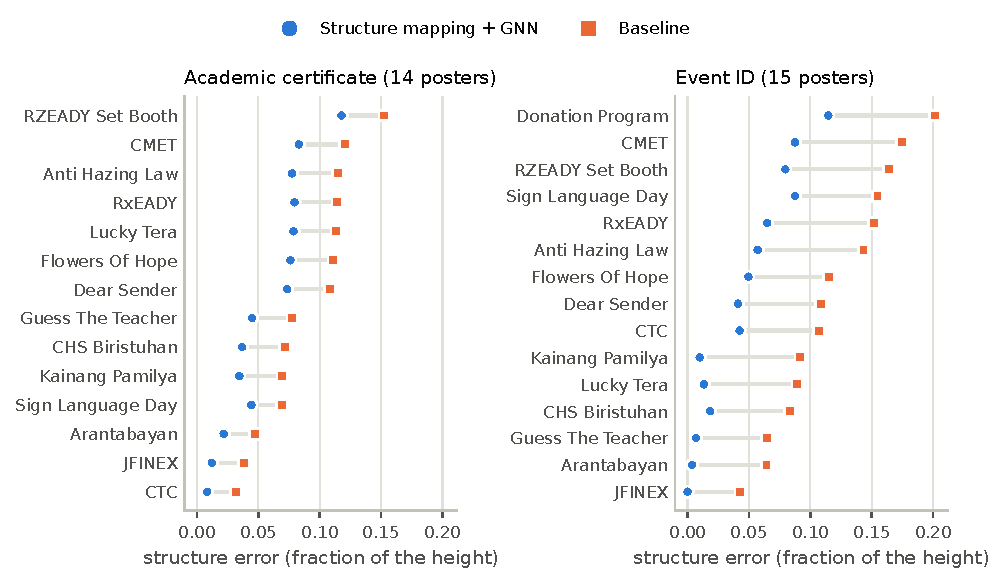
\includegraphics[width=0.92\textwidth]{figures/fig4_structure_error}
    \caption{Structure Error per Poster, Structure Mapping + GNN Against the Baseline}
    \label{fig:structure-error}
\end{figure}
% Source: results/figures/fig4_structure_error (notebooks/results_analysis.ipynb); per-poster
% values from results/experiment_log.json (structure_error_all).

Every poster with mappable roles had a lower structure error with structure mapping + GNN than with the baseline. The reduction was similar from poster to poster: 0.023 to 0.037 on certificates and 0.043 to 0.087 on event IDs. The remaining error varied more, from 0.008 to 0.118 on certificates and from 0.000 to 0.115 on event IDs.

The improvement was consistent across posters and was not driven by a few of them. The steady reduction showed that the mapping worked the same way on every master, while the remaining error depended on how far each master's arrangement was from what the target format's design rules allowed. Zhou, Xu, Ma, Ge, Jiang, and Xu [\citeyear{zhou2022cglgan}] conditioned layout generation on the composition of the poster image; ThemeSync conditioned the target layout on the master's structure directly, and this held across varied masters. A designer could expect the master's arrangement to carry over for most event posters, not only typical ones. The 16 posters came from school organizations. Every mappable poster gained from the structure mapping.

% =====================================================================
\clearpage
\section{Objective 2: Reactive Layout Synthesis}

The second specific objective was to develop a Reactive Layout Synthesis engine that used a Bi-directional State Machine and the Cassowary algorithm to solve Constraint Satisfaction Problems, propagating manual Hard Constraints in real time while preserving the global layout state.

\subsection{Constraint Satisfaction}

\ref{tab:rated-f1} presented the F1-score and text fit of the 64 rated layouts, read from the printed files.

\begin{table}[H]
\centering
\caption{Structural Accuracy and Text Fit of the 64 Rated Layouts}
\label{tab:rated-f1}
\setlength{\tabcolsep}{4pt}
\begin{tabular}{l c c c c}
\hline
 & \multicolumn{2}{c}{\textbf{Certificate}} & \multicolumn{2}{c}{\textbf{Event ID}} \\
 & \textbf{Mapping + GNN} & \textbf{Baseline} & \textbf{Mapping + GNN} & \textbf{Baseline} \\ \hline
F1-score & 1.0 (all) & 1.0 (all) & 1.0 (all) & 1.0 (all) \\
Reading order kept & 16 & 16 & 16 & 16 \\
All text within its box & 16 & 16 & 14 & 14 \\
Text over other content & 0 & 0 & 0 & 0 \\
Smallest text at print size & 7.8 pt & 7.8 pt & 6.5 pt & 6.5 pt \\ \hline
\end{tabular}
\end{table}
% Source: results/rated_layouts_check.json (notes §3.44).

All 64 layouts reached an F1-score of 1.0, and none of their 384 candidates broke a constraint. On two event IDs, a header line was 6 to 19 pixels wider than its box, inside the card's panel. A crowded test edit lowered the F1-score to 0.90.

The solver kept every layout valid, so designers had no overlaps to fix. Cassowary satisfies required constraints and relaxes only preferences, as Badros, Borning, and Stuckey [\citeyear{Badros2001Cassowary}] designed it to do. The F1-score checks boxes, not text, and was 1.0 in both conditions, so it could not separate them. Every rated layout was structurally valid.

\clearpage
The synthetic templates were filled with extreme payloads (\ref{tab:stress}): fields at 25\% to 100\% of their maximum length, one character over it, and 1 to 10 signature blocks.

\begin{table}[H]
\centering
\caption{Stress Test of the Synthetic Templates}
\label{tab:stress}
\setlength{\tabcolsep}{4pt}
\begin{tabular}{>{\raggedright\arraybackslash}p{0.32\textwidth} >{\raggedright\arraybackslash}p{0.28\textwidth} >{\raggedright\arraybackslash}p{0.28\textwidth}}
\hline
\textbf{Condition} & \textbf{Academic Certificate} & \textbf{Event ID} \\ \hline
Every field at its maximum (real words) & All text fit & The organization header overflowed \\
First failure (real words) & None & Organization header from 49 of 90 characters \\
First failure (one unbroken string) & Citation from 98 of 150 characters & Event details from 51 of 80 characters \\
Maximum + 1 character & Rejected (all 7 fields) & Rejected (all 5 fields) \\
Reading order & Held in every run & Held in every run \\
F1-score & 1.0 in every length run & 1.0 in every run \\
Signature blocks & Clean up to 5; overlapping from 6 (F1 0.92) & --- \\ \hline
\end{tabular}
\end{table}
% Source: results/stress_test.json (notes §3.42). Text fit used the font's actual glyph widths.
% Smallest text at print size (event ID at A6, certificate at US Letter landscape): 7.8 pt and 6.5 pt.

The boxes stayed apart, on the canvas, and in order in every run, and the schema rejected every over-length field. The certificate's name shrank from 31.3 to 13.5 points to fit 60 characters, while event ID header lines over 48 characters overflowed. Overflowing runs still scored an F1-score of 1.0.

The solver held at every length; the limits were in text fitting, since the header's box did not shrink its text. Jiang, Stuerzlinger, Zwicker, and Lutteroth [\citeyear{Jiang2020ORCSolver}] let adaptive layouts switch arrangements with OR-constraints, while ThemeSync's templates were fixed. Long organization names and more than five signatories need handling. The test covered the two synthetic templates. The engine was robust, with two text-fit limits.

\clearpage
\subsection{Propagation of Manual Hard Constraints}

The Bi-directional State Machine recorded every terminal edit as a new, immutable state in the JSON state chain. Simulated moves, resizes, and locks were kept exactly through every later re-solve, with no overlap among the surrounding elements, and every re-solve of a session's chain was checked against the edits made before it. Undo and redo restored earlier states by appending them as new states, so the chain stayed append-only. Text edits were re-validated against the content schema before they were accepted. Each edit was made on the dashboard's canvas and produced exactly one terminal event, verified in a real browser.
% Sources: evaluate.py (test_hard_constraints_preserved), layout_report.retention_check (notes §3.28, §3.32).

The engine propagated manual Hard Constraints without overwriting earlier edits. Because each edit became a required constraint and a new state, a re-solve could move only the elements the designer had not fixed. Generative layout models recalculate the whole layout and can overwrite manual changes \cite{Shi2023Survey}; the state chain instead kept every edit, in line with the human-in-the-loop co-design that He, Huang, and Wang [\citeyear{He2022iPLAN}] demonstrated with iPLAN and with the bi-directional state machine of Liang, McGee, Menassa, and Kamat [\citeyear{Liang2020Bidirectional}]. This addressed the destructive state management identified in Chapter 1. The checks used simulated sessions, not designers' own sessions. The engine met the requirement to preserve manual edits.

\clearpage
\subsection{Real-Time Performance}

Latency was measured over 34 editing sessions of 40 edits each (1,360 edits) on the 16 posters in both formats and on the synthetic theme (\ref{tab:latency}). The solver timing was the constraint recalculation, and the full edit was the state synchronization.

\begin{table}[H]
\centering
\caption{Latency of the Designer's Edits}
\label{tab:latency}
\begin{tabular}{l c c c c c c}
\hline
\textbf{Timing} & \textbf{Edits} & \textbf{Median} & \textbf{95th Pct.} & \textbf{Max} & \textbf{$\leq$ 0.1 s} & \textbf{$\leq$ 1.0 s} \\ \hline
Solver & 1,012 & 0.4 ms & 0.8 ms & 95.9 ms$^{a}$ & 100\% & 100\% \\
Full edit & 1,360 & 90 ms & 176 ms & 206 ms & 61\% & 100\% \\
\quad Certificate & 680 & 146 ms & 182 ms & 206 ms & 29\% & 100\% \\
\quad Event ID & 680 & 86 ms & 103 ms & 159 ms & 93\% & 100\% \\ \hline
\multicolumn{7}{p{0.80\textwidth}}{\footnotesize Solver: the constraint recalculation. Full edit: the state synchronization (re-solve, re-score, re-draw, and save). $^{a}$One solve paused by the operating system; every other solve took at most 1.9 ms. The browser's redraw of the page is not included.}
\end{tabular}
\end{table}
% Source: results/latency_benchmark.json (notes §3.43, §3.47), measured after the renderer's image
% cache (§3.47), which left every output byte-identical. Before it: full-edit median 157 ms, 22% within 0.1 s.
% Means: solver 0.53 ms (SD 3.01), full edit 90.6 ms (SD 57.5).

Every recalculation finished within 0.1 seconds, and all but one, paused by the operating system, within 1.9 milliseconds. Every full edit finished within 1.0 second, and 61\% within 0.1 seconds. Full edits took longer on certificates than on event IDs (median 146 against 86 milliseconds).

The solver responded instantly, and every full edit stayed within the limit for uninterrupted work. Most of a full edit's time went to re-scoring legibility against the poster's background, and certificates have more elements and a larger canvas. Against the limits of Nielsen [\citeyear{nielsen1993usability}], the solver was instantaneous and the full edit did not interrupt the task, in line with the interactive purpose of Cassowary \cite{Badros2001Cassowary} and the real-time constraint-based layout of Li, Li, Fu, and Cai [\citeyear{Li2024SMT}]. A designer could edit without waiting. Latency was measured on one workstation, without the browser's redraw. The engine met the real-time requirement.

\clearpage
\ref{fig:latency} presented the cumulative share of edits by time, with the 0.1-second and 1.0-second limits.

\begin{figure}[H]
    \centering
    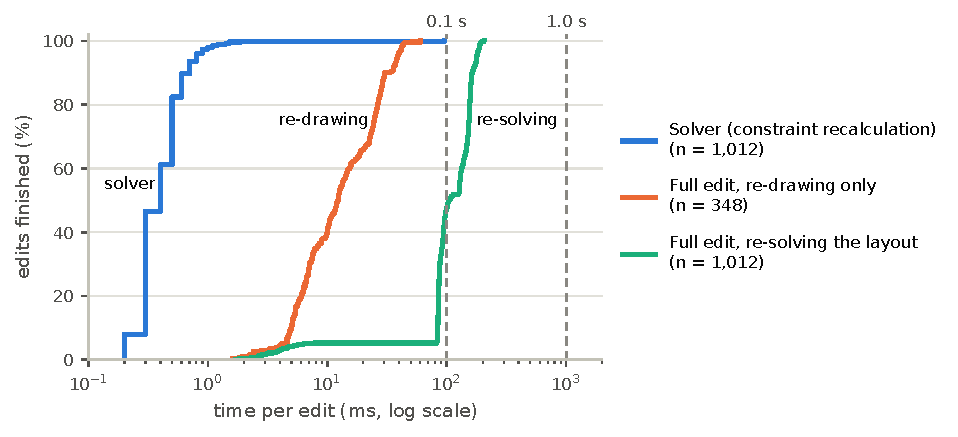
\includegraphics[width=0.92\textwidth]{figures/fig4_latency}
    \caption{Cumulative Share of Edits by Time, With the 0.1-Second and 1.0-Second Limits}
    \label{fig:latency}
\end{figure}

Edits that only re-drew the canvas (text edits, typography changes, undo, redo, restore, and candidate selections) all finished within 0.1 seconds, with a median of 12 milliseconds. Edits that re-solved the layout (moves, resizes, and locks) had a median of 105 milliseconds, and 48\% of them finished within 0.1 seconds. Opening a layout, which ran every stage of the pipeline, took a median of 3.4 seconds. The timings included an image cache that left the layouts byte-identical.

The edits fell into two groups: re-draws, which were instant, and re-solves, which met the 0.1-second limit about half the time. A full edit on the synthetic theme took about 4 milliseconds, so re-scoring legibility against the poster's background, not the solver, set the time of the re-solves. Nielsen [\citeyear{nielsen1993usability}] placed the limit for a response that feels instantaneous at 0.1 seconds; about half of the re-solves fell just above it. Cheaper legibility scoring would bring most of them under 0.1 seconds. Opening a layout took seconds, but only once per layout. Real-time editing was achieved, with room to make re-solves faster.

% =====================================================================
\clearpage
\section{Objective 3: Heuristic Evaluation and Expert Validation}

The third specific objective was to evaluate the generated layouts with a mathematically calibrated Heuristic Fitness Function that ranked parallel design candidates, followed by a quantitative human-expert validation.

\subsection{Ranking of Parallel Candidates}

\ref{tab:fitness} presented the fitness of the output layouts, each chosen from six candidates solved by Cassowary and scored by Formula 3.11.

\begin{table}[H]
\centering
\caption{Heuristic Fitness of the Output Layouts on the 16 Unseen Posters (Means)}
\label{tab:fitness}
\begin{tabular}{l l c c c}
\hline
\textbf{Format} & \textbf{Condition} & \textbf{$F_{layout}$} & \textbf{$P_{whitespace}$} & \textbf{$P_{legibility}$} \\ \hline
Certificate & Mapping + GNN & 0.0125 & 0.0108 & 0.0011 \\
 & Baseline & 0.0126 & 0.0108 & 0.0012 \\ \hline
Event ID & Mapping + GNN & 0.1633 & 0.1508 & 0.0083 \\
 & Baseline & 0.1583 & 0.1508 & 0.0050 \\ \hline
\multicolumn{5}{p{0.80\textwidth}}{\footnotesize Lower is better. $P_{collision} = 0$ and $P_{alignment} \approx 0$ in every run.}
\end{tabular}
\end{table}
% Source: results/experiment_log.json, run 20261006_195534. Mapping only: certificate 0.0125/0.0108/0.0011,
% event ID 0.1621/0.1508/0.0075. Over the 32 pairs, structure mapping + GNN
% scored higher in 15, lower in 7, the same in 10; means 0.0879 (SD 0.0791) and 0.0855 (SD 0.0766).

The two conditions scored the same on 10 of the 16 certificates, and the baseline scored lower (better) on event IDs through the legibility penalty. Over the 32 pairs, the Wilcoxon signed-rank test favored the baseline ($p = 0.030$, $r = +0.53$).

The fitness function slightly favored the baseline. The legibility term penalized text placed over the poster's artwork, while the whitespace term was equal in both conditions. Like the energy model of O'Donovan, Agarwala, and Hertzmann [\citeyear{ODonovan2014Layouts}], Formula 3.11 combined penalties for overlap, whitespace, and misalignment, but none of its terms measured where the space went or how closely the output followed the master. The fitness function measured little of what separated the conditions.

\clearpage
In an earlier run in which the fitness function alone chose the output, ``classic centered'' won 14 of the 16 certificates because the top candidates tied exactly, and ``left-aligned'' won all 16 event IDs by a small, steady margin. The master's composition, read from the detected elements, then chose the archetype, and the fitness function ranked the candidates within it (\ref{tab:archetypes}).

\begin{table}[H]
\centering
\caption{Layout Archetypes Selected From the Masters' Compositions (16 Posters)}
\label{tab:archetypes}
\begin{tabular}{l c l c}
\hline
\multicolumn{2}{c}{\textbf{Certificate}} & \multicolumn{2}{c}{\textbf{Event ID}} \\ \hline
Classic centered & 11 & Classic centered & 9 \\
Header banner & 2 & Floating card & 2 \\
Art column & 2 & Full-width band & 2 \\
Left-aligned & 1 & Left-aligned & 3 \\ \hline
\end{tabular}
\end{table}
% Source: results/experiment_log.json (winner_label); same archetype in both conditions of every poster.

The 16 posters received four archetypes in each format, and both conditions received the same archetype on every poster. The chosen candidate did not always have the lowest fitness: the art column scored about 0.076 against 0.003 for the classic layout, and the floating card about 0.187 against 0.149 for the left-aligned layout.

The master's composition, not the fitness function, gave the outputs their variety. The fitness function could not tell the archetypes apart well, since its top candidates tied or differed by small, constant margins. Zhou, Xu, Ma, Ge, Jiang, and Xu [\citeyear{zhou2022cglgan}] conditioned layout generation on the composition of the poster image; ThemeSync applied the same idea by taking the archetype from the master's composition. A fitness function alone was not enough to choose among layout types. Choosing by composition meant accepting some candidates with a higher fitness. Each poster received a layout type that followed its master.

\clearpage
\subsection{Calibration of the Fitness Weights}

The weights of Formula 3.11 were set by the priority rule of Chapter 3 and calibrated on the 64 rated runs with criteria fixed in advance: a change to one weight (by a factor of 0.25 to 4) was kept only if the selected layouts improved on a design rule and worsened on none. \ref{tab:calibration} presented how many selections changed when one weight was scaled.

\begin{table}[H]
\centering
\caption{Selected Layouts That Changed When One Fitness Weight Was Scaled (of 64)}
\label{tab:calibration}
\begin{tabular}{l c c c c c}
\hline
\textbf{Weight (Deployed Value)} & \textbf{$\times 0$} & \textbf{$\times 0.25$} & \textbf{$\times 0.5$} & \textbf{$\times 2$} & \textbf{$\times 4$} \\ \hline
$\alpha$, collision (50) & 0 & 0 & 0 & 0 & 0 \\
$\beta$, alignment (2) & 0 & 0 & 0 & 0 & 0 \\
$\gamma$, whitespace (1) & 11 & 1 & 1 & 1 & 0 \\
$\delta$, legibility (1.5) & 5 & 1 & 1 & 0 & 0 \\ \hline
\multicolumn{6}{p{0.80\textwidth}}{\footnotesize $\times 0$ removed the term; the other weights stayed at their deployed values. Every setting kept the constraints in all 64 runs.}
\end{tabular}
\end{table}
% Source: results/weight_calibration.json, analysis.deployed.sensitivity (notes §3.33);
% results/r_target_analysis.json (notes §3.46).

The loop kept no change, which confirmed the deployed weights. Halving or doubling any weight changed at most 1 of the 64 selections; removing the whitespace or legibility term changed 11 or 5. Of the 48 runs with two candidates of the chosen archetype, 22 tied exactly. A whitespace target taken from each master instead of 0.65 would have changed 2 layouts. The calibration ran before any rating was analyzed.

The weights were stable. They mattered little because no candidate overlapped, the alignment penalty was near zero, and candidates of one archetype had nearly the same whitespace. O'Donovan, Agarwala, and Hertzmann [\citeyear{ODonovan2014Layouts}] learned the weights of their energy terms from example designs; here, the weights were not the deciding factor. Improving the fitness function would need new terms, not new weights. The calibration used the formula's own terms, not the experts' ratings. The weights were confirmed and robust.

\clearpage
\subsection{Expert Validation}

Four professional designers rated the 64 layouts on the three parameters of \ref{tab:mos-rating-scale} without knowing the conditions (768 ratings). The rated pages of ANTI\_HAZING\_LAW carried two extraction defects in both conditions. The analysis followed the statistical treatment of Chapter 3, fixed in advance (\ref{tab:mos}).

\begin{table}[H]
\centering
\caption{Mean Opinion Score by Format, Condition, and Parameter}
\label{tab:mos}
\setlength{\tabcolsep}{4pt}
\begin{tabular}{l l c c c c}
\hline
\textbf{Format} & \textbf{Condition} & \textbf{Hierarchy} & \textbf{Brand} & \textbf{Whitespace} & \textbf{Overall} \\ \hline
Certificate & Mapping + GNN & 3.88 $\pm$ 1.05 & 3.56 $\pm$ 1.02 & 3.06 $\pm$ 1.28 & 3.50 $\pm$ 0.89 \\
 & Baseline & 3.73 $\pm$ 1.20 & 3.78 $\pm$ 1.00 & 3.81 $\pm$ 1.19 & 3.78 $\pm$ 0.98 \\ \hline
Event ID & Mapping + GNN & 3.34 $\pm$ 1.01 & 3.38 $\pm$ 1.15 & 2.78 $\pm$ 1.06 & 3.17 $\pm$ 0.85 \\
 & Baseline & 3.72 $\pm$ 1.02 & 3.62 $\pm$ 1.05 & 3.73 $\pm$ 1.07 & 3.69 $\pm$ 0.87 \\ \hline
Both & Mapping + GNN & 3.61 $\pm$ 1.06 & 3.47 $\pm$ 1.09 & 2.92 $\pm$ 1.18 & 3.33 $\pm$ 0.89 \\
 & Baseline & 3.73 $\pm$ 1.11 & 3.70 $\pm$ 1.02 & 3.77 $\pm$ 1.13 & 3.73 $\pm$ 0.93 \\ \hline
\multicolumn{6}{p{0.92\textwidth}}{\footnotesize Mean $\pm$ SD of 64 ratings per cell for one format and 128 for both. The overall score is the mean of the three parameters.}
\end{tabular}
\end{table}
% Source: results/phase4_analysis.json, q1_describe (notes §3.49). All layouts: Hierarchy 3.67 (SD 1.08),
% Brand 3.59 (1.06), Whitespace 3.35 (1.23), overall 3.53 (0.93).

The overall MOS was 3.53 (SD 0.93), between Acceptable and Good. The baseline was rated higher on every parameter and overall (3.73 against 3.33), most on Constraint and Whitespace Harmony (3.77 against 2.92) and least on Visual Hierarchy Preservation (3.73 against 3.61). The one exception was Visual Hierarchy Preservation on certificates (3.88 for structure mapping + GNN against 3.73).

The experts preferred the baseline, mostly for its use of space; keeping the master's positions did not make the hierarchy clearer. O'Donovan, Agarwala, and Hertzmann [\citeyear{ODonovan2014Layouts}] called white space ``fundamental for readability and aesthetics,'' and the ratings reflected this. Following a master's structure did not by itself earn higher ratings. The MOS came from 16 posters and four experts. The baseline was preferred overall.

\clearpage
\ref{fig:rating-distribution} presented how often each rating was given, by parameter and condition.

\begin{figure}[H]
    \centering
    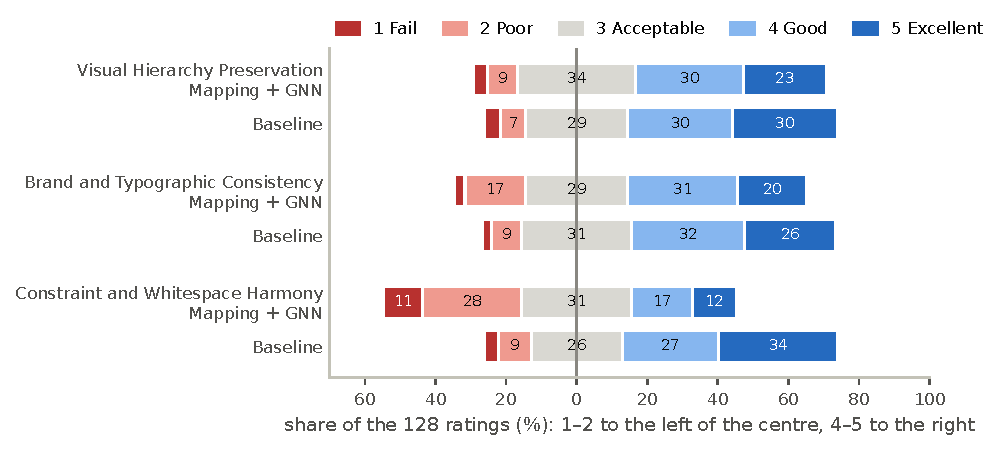
\includegraphics[width=\textwidth]{figures/fig4_rating_distribution}
    \caption{Distribution of the Ratings by Parameter and Condition}
    \label{fig:rating-distribution}
\end{figure}
% Source: results/phase4_analysis.json, q1_rating_counts.

Across the three parameters, structure mapping + GNN received 92 ratings of 1 or 2 and 71 ratings of 5, out of 384. The baseline received 46 ratings of 1 or 2 and 114 ratings of 5. On Constraint and Whitespace Harmony alone, structure mapping + GNN received 50 ratings of 1 or 2, against 17 for the baseline.

Structure mapping + GNN received twice as many low ratings as the baseline and fewer top ratings. Most of the extra low ratings were on Constraint and Whitespace Harmony, so a specific weakness, not a general one, drove the difference. Patnaik, Jain, Krishnamurthy, and Sarkar [\citeyear{Patnaik2025AesthetiQ}] aligned layout generation with human aesthetic preferences, and the distribution showed why such preferences have to be measured directly: the objective checks rated both conditions as equally valid. Fixing the spacing would address most of the low ratings. The counts pooled four experts who differed in leniency. The low ratings concentrated on whitespace.

\clearpage
\ref{tab:kendall} presented the agreement of the four experts on the order of the 64 layouts.

\begin{table}[H]
\centering
\caption{Agreement of the Four Experts Over the 64 Layouts (Kendall's $W$)}
\label{tab:kendall}
\begin{tabular}{l c c c}
\hline
\textbf{Parameter} & \textbf{$W$} & \textbf{$\chi^2$ (df = 63)} & \textbf{$p$} \\ \hline
Visual Hierarchy Preservation & 0.579 & 145.9 & $< 0.001$ \\
Brand and Typographic Consistency & 0.477 & 120.2 & $< 0.001$ \\
Constraint and Whitespace Harmony & 0.570 & 143.5 & $< 0.001$ \\ \hline
\textbf{Overall} & \textbf{0.630} & \textbf{158.7} & $< 0.001$ \\ \hline
\end{tabular}
\end{table}
% Source: results/phase4_analysis.json, q2_kendall_w; ICC and alpha from "sensitivity".

On the scale of Schmidt [\citeyear{schmidt1997managing}], Kendall's $W$ showed moderate agreement overall (0.630), on Visual Hierarchy Preservation (0.579), and on Constraint and Whitespace Harmony (0.570), and weak agreement on Brand and Typographic Consistency (0.477). All four values were significant ($p < 0.001$). As a secondary check, the absolute agreement was lower: ICC(2,1) ranged from 0.16 to 0.31 and Krippendorff's $\alpha$ from 0.01 to 0.23. The experts' individual mean ratings ranged from 2.88 to 4.32.

The experts ranked the layouts similarly but used the scale differently. Kendall's $W$ measures agreement on order, while the ICC and Krippendorff's $\alpha$ measure agreement on the scores themselves, so the experts agreed on which layouts were better while some rated everything higher than others. Nielsen and Molich [\citeyear{nielsen1990heuristic}] found that single evaluators miss problems that several evaluators together find, which supported pooling the four experts; by the guidelines of Koo and Li [\citeyear{koo2016guideline}] and of Krippendorff [\citeyear{krippendorff2004content}], however, their absolute agreement was poor. The comparison between the conditions, which relied on the order within pairs, was therefore more dependable than the absolute MOS values. Only four experts rated, with no calibration round before the rating. The agreement was sufficient for comparing the conditions.

\clearpage
\ref{tab:wilcoxon} presented the Wilcoxon signed-rank tests on the 32 pairs, at a significance level of 0.05.

\begin{table}[H]
\centering
\caption{Wilcoxon Signed-Rank Tests on the 32 Pairs}
\label{tab:wilcoxon}
\setlength{\tabcolsep}{4pt}
\begin{tabular}{l c c c c c c c}
\hline
\textbf{Parameter} & \textbf{B $>$ M} & \textbf{M $>$ B} & \textbf{Equal} & \textbf{Median Diff.} & \textbf{$T$} & \textbf{$p_{Holm}$} & \textbf{$r$} \\ \hline
Overall (main test) & 25 & 2 & 5 & $-0.42$ & 9.5 & $< 0.001$ & $-0.95$ \\
Hierarchy & 16 & 7 & 9 & $-0.13$ & 88.5 & 0.127 & $-0.36$ \\
Brand & 22 & 5 & 5 & $-0.25$ & 50.0 & $< 0.001$ & $-0.74$ \\
Whitespace & 26 & 2 & 4 & $-1.00$ & 4.0 & $< 0.001$ & $-0.98$ \\ \hline
\multicolumn{8}{p{0.92\textwidth}}{\footnotesize B $>$ M, M $>$ B: pairs rated higher for the baseline or for structure mapping + GNN. A negative $r$ favors the baseline. Two-sided tests, Holm-corrected over the four tests.}
\end{tabular}
\end{table}
% Source: results/phase4_analysis.json, q3_q9_wilcoxon. Exact p (Holm): overall 4.6e-5, Brand 9.7e-4, Whitespace 2.2e-5.
% Sensitivity: paired t-test overall t(31) = -6.57, p < 0.001; Bonferroni changed no conclusion.

The experts rated the baseline significantly higher overall, the main test ($T = 9.5$, $p_{Holm} < 0.001$, $r = -0.95$, a large effect), and on Brand and Typographic Consistency and Constraint and Whitespace Harmony. Visual Hierarchy Preservation showed no significant difference ($p_{Holm} = 0.127$). The paired t-test and the Bonferroni correction agreed. Without the one pair whose layouts rendered identically, Visual Hierarchy Preservation reached significance ($p_{Holm} = 0.046$), so that result was borderline.

The preference for the baseline was significant, large, and robust, the opposite of the expected direction. Because the GNN's output was registered to the master's anchors, the difference reflected mainly the structure mapping. Zhou, Xu, Ma, Ge, Jiang, and Xu [\citeyear{zhou2022cglgan}] had designers judge generated posters alongside objective measures; here, the F1-score was equal in both conditions, yet the experts separated them, which supported human evaluation as practiced by Li, Liu, Feng, Zhu, Li, Zhang, Lv, Zhu, Shen, Lin, and Shao [\citeyear{li2023radm}]. The structure mapping needs a step that evens out the spacing. The baseline lacked both the mapping and the GNN, so the test could not isolate the GNN. The expert validation did not support the structure mapping + GNN condition.

\clearpage
\ref{fig:pairs} presented the overall MOS of each of the 32 pairs.

\begin{figure}[H]
    \centering
    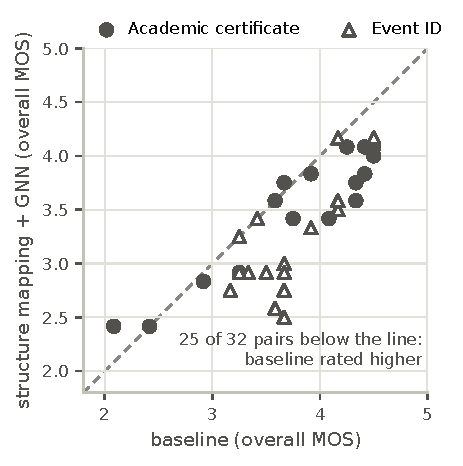
\includegraphics[width=0.55\textwidth]{figures/fig4_pairs}
    \caption{Overall Mean Opinion Score of the 32 Pairs}
    \label{fig:pairs}
\end{figure}

Of the 32 pairs, 25 lay below the line of equal scores, in favor of the baseline. In exploratory analyses, which were added after the planned tests and not corrected, each of the four experts rated the baseline higher on average, by 0.15 to 0.75 points. Without ANTI\_HAZING\_LAW, whose rated pages carried two defects, the conclusions were unchanged (overall $p_{Holm} < 0.001$, $r = -0.95$; Visual Hierarchy Preservation $p = 0.153$).

The preference for the baseline was spread across the pairs and the experts. It did not depend on a few posters, on one expert, or on the defective poster. As in the method of ITU-T P.800 \cite{itut1996p800}, the MOS averaged several raters, and the per-expert results showed that the average was not driven by any one of them. The result can be taken as a consistent judgment of these experts, not an artifact of one rater or poster. The per-expert and exclusion analyses were exploratory. The preference for the baseline was consistent.

\clearpage
A post hoc comparison measured the spacing of the rated layouts (\ref{tab:spacing}). The largest gap and the stack spread were fractions of the layout's height, and the gap CV was the coefficient of variation of the gaps.

\begin{table}[H]
\centering
\caption{Spacing of the Rated Layouts (Post Hoc)}
\label{tab:spacing}
\begin{tabular}{l c c c c}
\hline
\textbf{Measure} & \textbf{Mapping + GNN} & \textbf{Baseline} & \textbf{$\rho$} & \textbf{$p$} \\ \hline
Largest gap & 0.072 $\pm$ 0.057 & 0.020 $\pm$ 0.003 & $-0.42$ & 0.017 \\
Gap CV & 0.47 $\pm$ 0.44 & 0.00 $\pm$ 0.00 & $-0.42$ & 0.017 \\
Stack spread & 0.816 $\pm$ 0.054 & 0.746 $\pm$ 0.025 & $-0.45$ & 0.010 \\ \hline
\multicolumn{5}{p{0.80\textwidth}}{\footnotesize Mean $\pm$ SD over the 32 layouts of each condition. $\rho$: Spearman correlation over the 32 pairs between the change in the measure (structure mapping + GNN minus baseline) and the change in overall MOS; exploratory and uncorrected.}
\end{tabular}
\end{table}
% Source: results/phase4_posthoc.json (notes §3.49).

Structure mapping + GNN spread the elements over more of the height (0.816 against 0.746) and left larger, uneven gaps (largest gap 0.072 against 0.020; gap CV 0.47 against 0.00). The baseline stacked the elements with even gaps. The pairs in which the gaps grew the most lost the most MOS (Spearman's $\rho$ from $-0.42$ to $-0.45$, $p$ from 0.010 to 0.017).

Uneven spacing was the most likely reason for the lower ratings. Structure mapping placed the logo row, header, title, and details at their relative positions on the master, and because a poster has different proportions from a certificate or an event ID, these positions opened large gaps in the target, such as an empty band between the header and the title. O'Donovan, Agarwala, and Hertzmann [\citeyear{ODonovan2014Layouts}] penalized whitespace imbalance in their energy model, whereas the whitespace term of Formula 3.11 measured only the amount of empty space. The anchored positions should be balanced with an even distribution of the remaining space, for example by redistributing the gaps after anchoring. This analysis was exploratory and correlational, so it did not prove that spacing caused the lower ratings. Spacing explained the difference better than any measure the system used.

\clearpage
\ref{fig:spacing-vs-mos} presented the change in the largest gap against the change in overall MOS for the 32 pairs.

\begin{figure}[H]
    \centering
    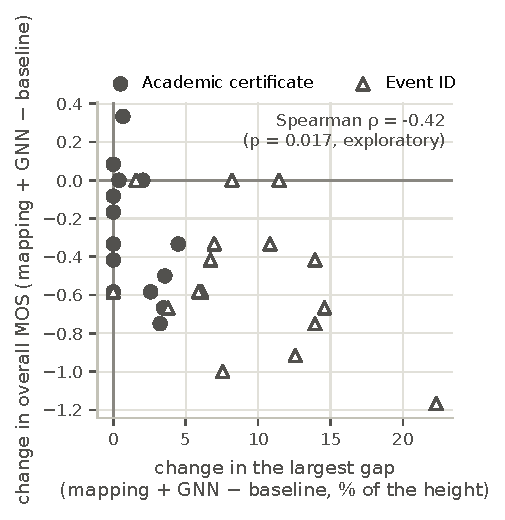
\includegraphics[width=0.52\textwidth]{figures/fig4_spacing_vs_mos}
    \caption{Change in the Largest Gap Against the Change in Overall MOS (Exploratory)}
    \label{fig:spacing-vs-mos}
\end{figure}
% Source: results/figures/fig4_spacing_vs_mos; results/phase4_posthoc.json.

The largest gap of structure mapping + GNN was larger than the baseline's in 23 of the 32 pairs and smaller in none. Larger increases in the gap went with larger losses of MOS. The difference in fitness between the two conditions did not follow the difference in MOS ($\rho = -0.20$, $p = 0.26$).

The experts' ratings followed the spacing, and the fitness function did not. The whitespace term of Formula 3.11 compares the ratio of empty to filled area, which is nearly the same for even and uneven gaps, so the fitness function could not see the change the experts reacted to. Guo, Fu, and Zhu [\citeyear{Guo2025Aesthetic}] turned design rules such as whitespace and visual density into objective metrics; the present result showed that such a metric has to capture how the space is distributed, not only how much of it there is. A term for the evenness of the gaps should be added to the fitness function. The figure showed a correlation from an exploratory analysis. The fitness function missed the spacing that the experts judged.

%=======================================================%
%%%%% Do not delete this part %%%%%%
\clearpage

\begin{center}
\textbf{Notes}
\end{center}
\printbibliography[heading=none]
\end{refsection}
